\documentclass[12pt,a4paper]{book}
\usepackage[utf8]{inputenc}
\usepackage[french]{babel}
\usepackage[T1]{fontenc}
\usepackage{amsmath}
\usepackage{amsfonts}
\usepackage{amssymb}
\usepackage[left=2cm,right=2cm,top=2cm,bottom=2cm]{geometry}
\usepackage{multirow}
\usepackage{graphicx}

\author{itchesside Raoul}
\begin{document}
\centering
\begin{table}[h!]%la précision sur le h! pour qu'il reste reste néccésairement sur une même page
\begin{tabular}{|c|c|c|c|}\hline
1&2&3&4\\
\hline
\multicolumn{2}{|c|}{blabla}&6&10\\\hline
&&9&11\\
\hline

\end{tabular}
\hspace{5cm}
\begin{tabular}{|c|c|c|c|}\hline
1&2&3&4\\
\hline
\multicolumn{2}{|c|}%fusion de deux collones ayant 2cm de large et contenant le message 'c'est ça'
{blabla}&6&10\\\cline{3-4}%puis on trace une ligne entre la 3è et la 4è colonne à l'endroit mis
\multicolumn{2}{|c|}{}
&9&11\\
\hline
\end{tabular}
\\
\\%crée des esoaces verticales
\\
\begin{tabular}{|c|c|c|c|}\hline
1&2&3&4\\
\hline
\multicolumn{2}{|c|}{bla}
&6&10\\
\hline
&B&9&11\\
\hline
\end{tabular}
\hspace{5cm}
\begin{tabular}{|c|c|c|c|}\hline
1&2&3&4\\
\hline
\multirow{2}{2cm}{C'est ça}%fusion de deux ligne ayant 2cm de large et contenant le message 'c'est ça'
&&6&10\\\cline{2-4}
&B&9&11\\
\hline

\end{tabular}
\label{Table}
\caption{Titre de tables}

\end{table}
%inserer une nouvelle page vierge

\newpage
\thispagestyle{empty}
la vie du bon coté

%insertion d'image
\begin{figure}[h]
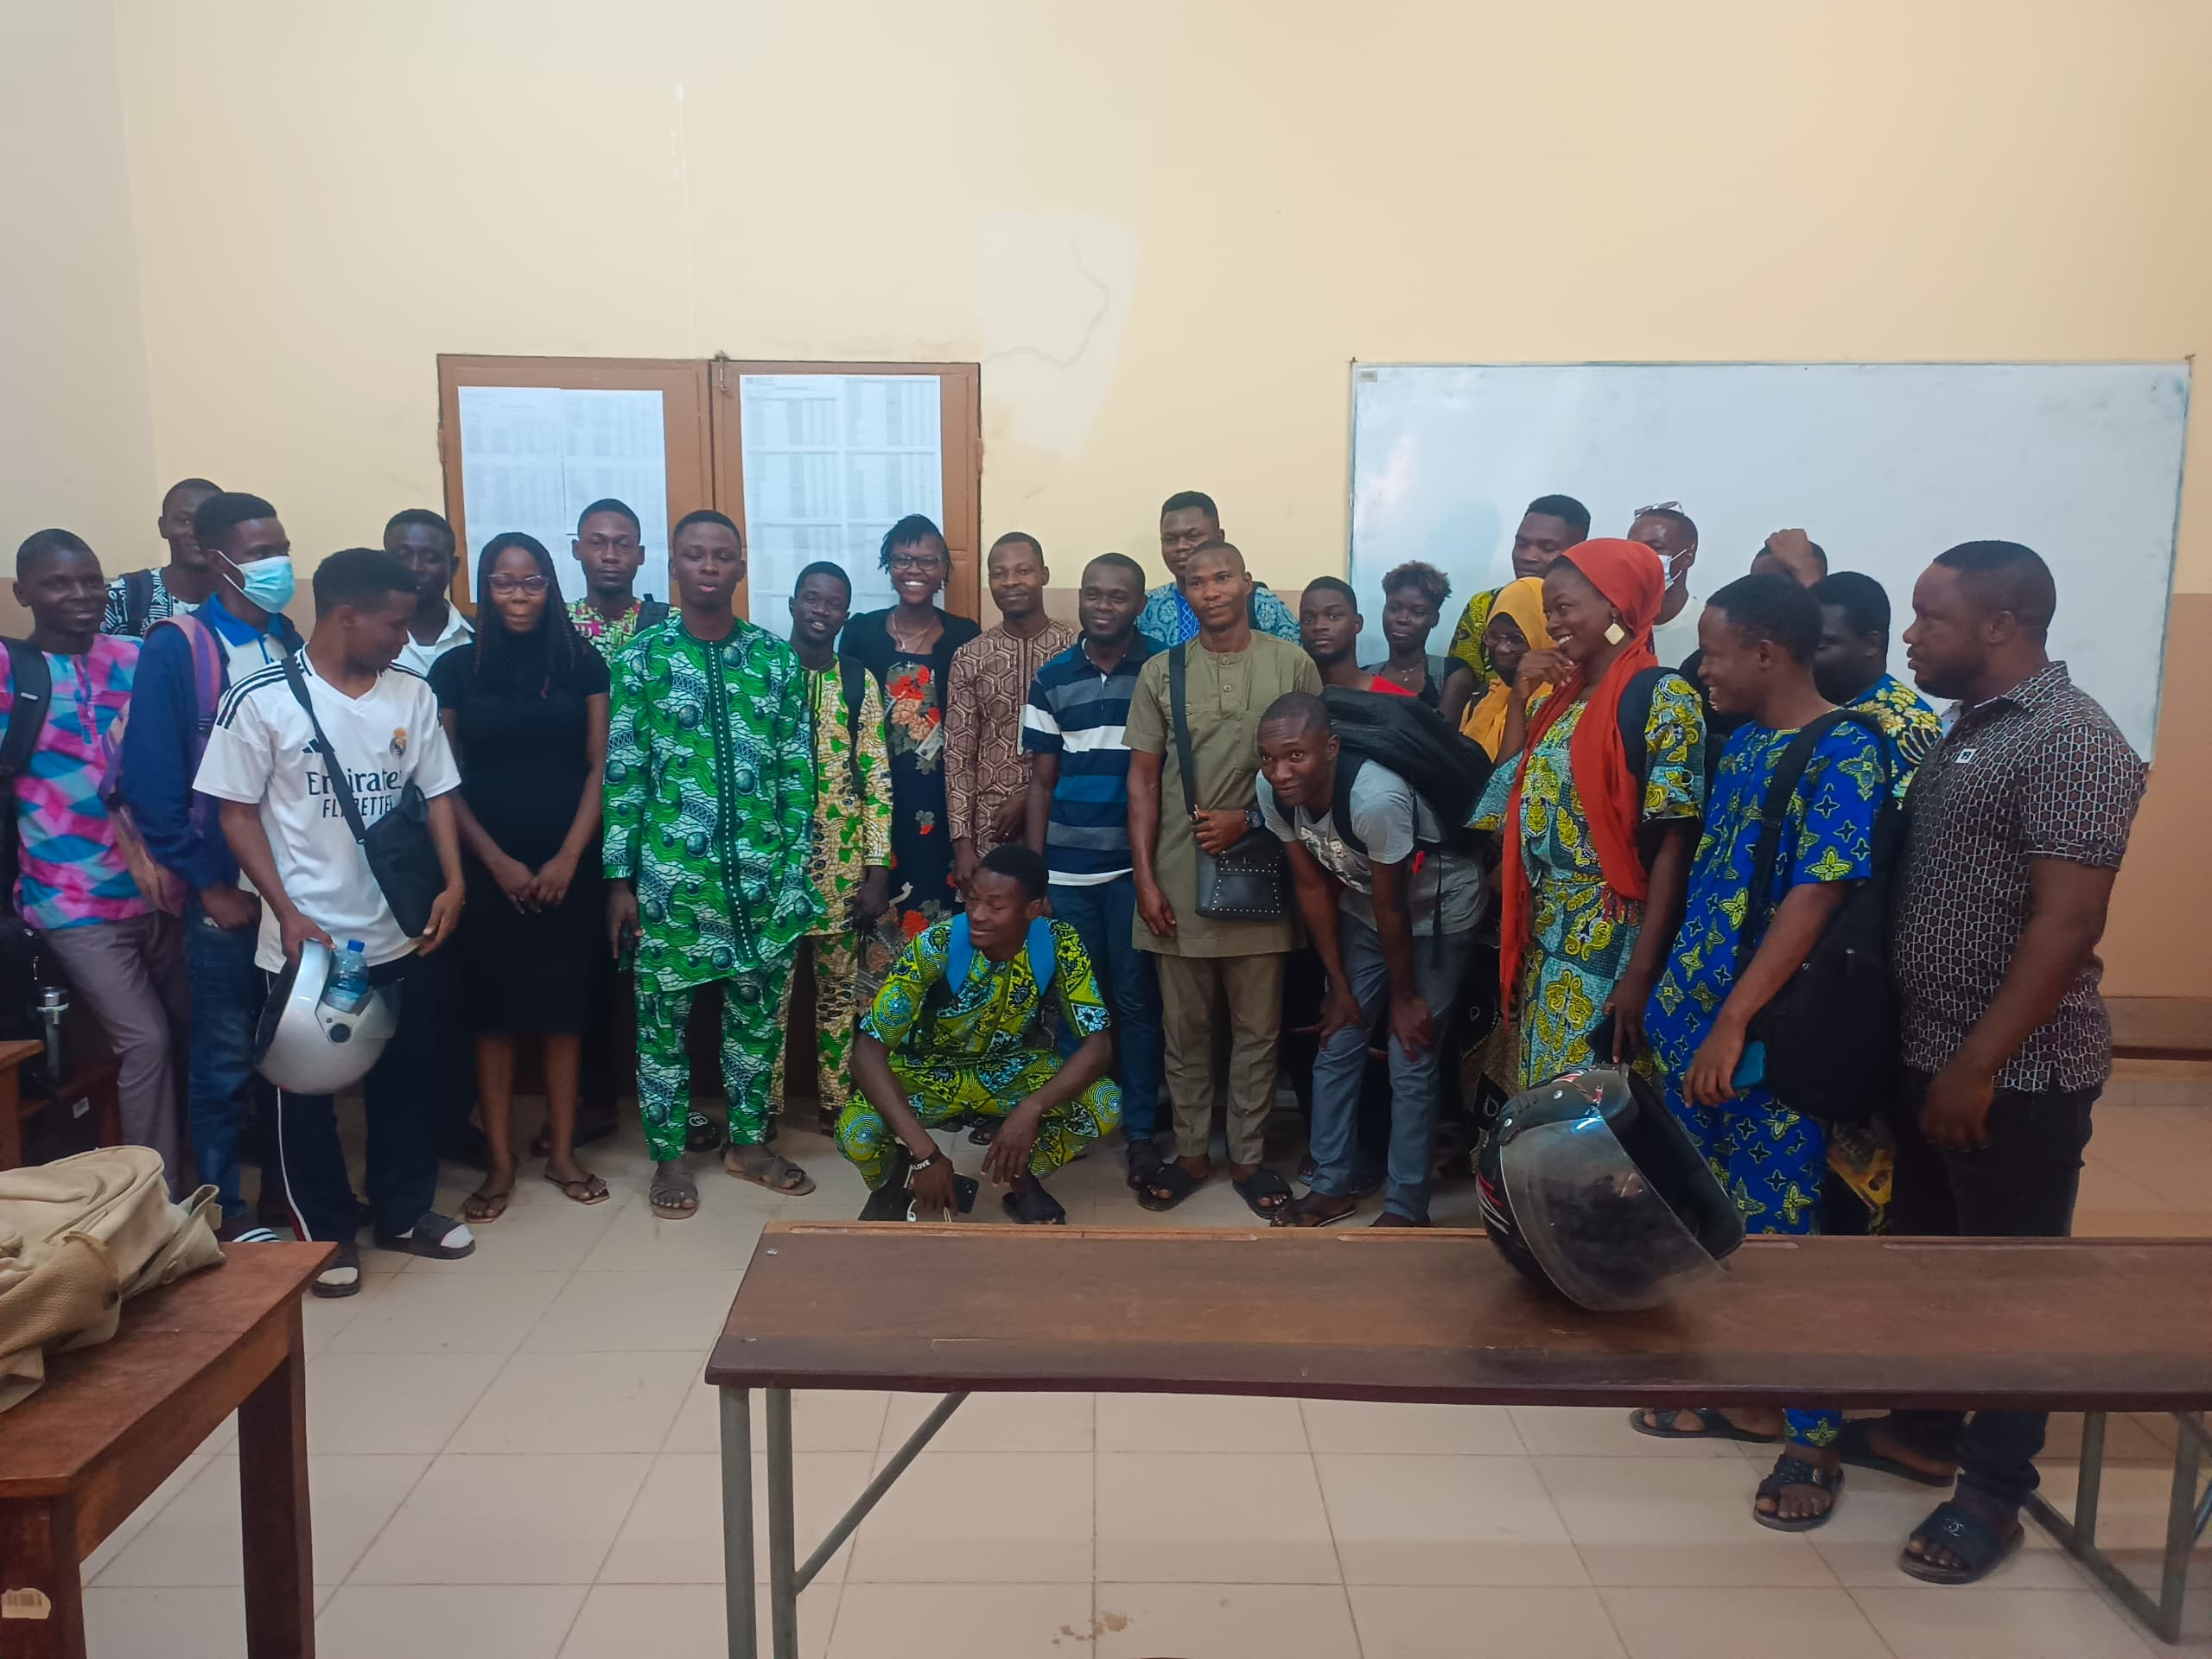
\includegraphics[scale=0.3]{aa.jpg}%scale correspond à l'échelle dont on veux le reduire 
\label{Photo}%nom à mettre en bas de l'image
\caption{photo de classe}%titre à ajouter à l'image
\end{figure}

\end{document}